\documentclass[tikz,border=3.14mm]{standalone}
\usepackage{pgfplots}

\begin{document}
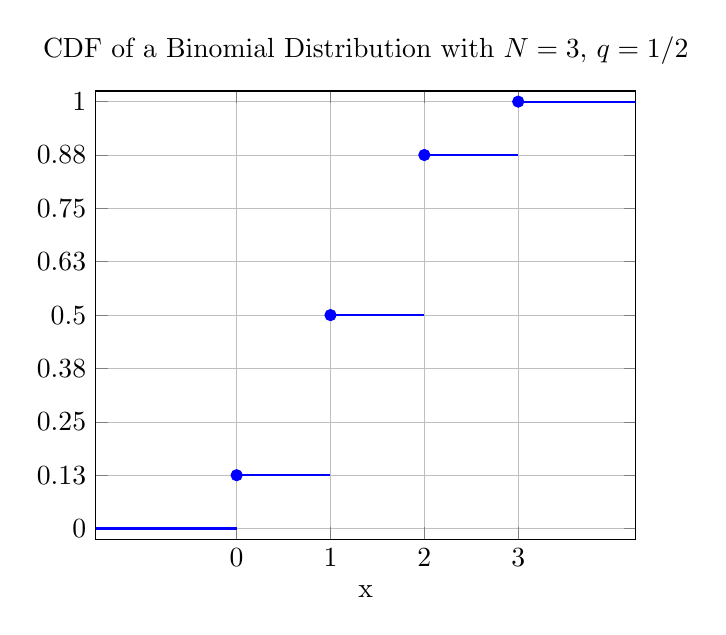
\begin{tikzpicture}
\begin{axis}[
    xlabel={x},
    title={CDF of a Binomial Distribution with $N=3$, $q=1/2$},
    xmin=-1.5, xmax=4.25,
    ymin=-0.025, ymax=1.025,
    xtick={0,1,2,3},
    ytick={0,0.125,0.25,0.375,0.5,0.625,0.75,0.875,1},
    grid=both,
    grid style={line width=.1pt, draw=gray!10},
    major grid style={line width=.2pt,draw=gray!50},
    % axis lines=middle,
]

% Horizontal lines
\addplot[blue, thick] coordinates {(-1.5,0) (0,0)};
\addplot[blue, thick] coordinates {(0,0.125) (1,0.125)};
\addplot[blue, thick] coordinates {(1,0.5) (2,0.5)};
\addplot[blue, thick] coordinates {(2,0.875) (3,0.875)};
\addplot[blue, thick] coordinates {(3,1) (4.25,1)};

% Dots
\addplot[blue,only marks,mark=*] coordinates {(0,0.125) (1,0.5) (2,0.875) (3,1)};

\end{axis}
\end{tikzpicture}
\end{document}
